\documentclass{report}
\usepackage{graphicx, tikz-cd, float, titlepic, booktabs} % Required for inserting images
\usepackage{pgfplots}
\usepackage{multicol}
\usepackage{makecell}
\pgfplotsset{compat=1.15}
\usepackage{mathrsfs}
\usetikzlibrary{arrows}
\usepackage{amsmath, amssymb, amsthm, amsfonts, siunitx, physics, gensymb}
\AtBeginDocument{\RenewCommandCopy\qty\SI}
\usepackage[version=4]{mhchem}
\usepackage[most,many,breakable]{tcolorbox}
\usepackage{xcolor, fancyhdr, varwidth}
\usepackage[Glenn]{fncychap}
%Options: Sonny, Lenny, Glenn, Conny, Rejne, Bjarne, Bjornstrup
\usepackage{hyperref, cleveref}
\usepackage{icomma, enumitem} %comma as decimal and continue enumerate with [resume]
\usepackage{plimsoll} %use standard state symbol with \stst
\usepackage[danish]{babel}
\renewcommand{\cellalign}{cl}
\renewcommand{\theadalign}{cl}
\renewcommand\theadfont{\bfseries}
%%%%%%%%%%%%%%%%%%%%%%%%%%%%%%
% SELF MADE COLORS
%%%%%%%%%%%%%%%%%%%%%%%%%%%%%%
\definecolor{myg}{RGB}{56, 140, 70}
\definecolor{myb}{RGB}{45, 111, 177}
\definecolor{myr}{RGB}{199, 68, 64}
\definecolor{mytheorembg}{HTML}{F2F2F9}
\definecolor{mytheoremfr}{HTML}{00007B}
\definecolor{mylenmabg}{HTML}{FFFAF8}
\definecolor{mylenmafr}{HTML}{983b0f}
\definecolor{mypropbg}{HTML}{f2fbfc}
\definecolor{mypropfr}{HTML}{191971}
\definecolor{myexamplebg}{HTML}{F2FBF8}
\definecolor{myexamplefr}{HTML}{88D6D1}
\definecolor{myexampleti}{HTML}{2A7F7F}
\definecolor{mydefinitbg}{HTML}{E5E5FF}
\definecolor{mydefinitfr}{HTML}{3F3FA3}
\definecolor{notesgreen}{RGB}{0,162,0}
\definecolor{myp}{RGB}{197, 92, 212}
\definecolor{mygr}{HTML}{2C3338}
\definecolor{myred}{RGB}{127,0,0}
\definecolor{myyellow}{RGB}{169,121,69}
\definecolor{myexercisebg}{HTML}{F2FBF8}
\definecolor{myexercisefg}{HTML}{88D6D1}
%%%%%%%%%%%%%%%%%%%%%%%%%%%%%%%%%%%%%%%%%%%%%%%%%%%%%%%%%%%%%%%%%%%%%%
% Box environments for theorems and problems
%%%%%%%%%%%%%%%%%%%%%%%%%%%%%%%%%%%%%%%%%%%%%%%%%%%%%%%%%%%%%%%%%%%%%
\setlength{\parindent}{1cm}
%================================
% Question BOX
%================================
\makeatletter
\newtcbtheorem{question}{Opgave}{enhanced,
	breakable,
	colback=white,
	colframe=myb!80!black,
	attach boxed title to top left={yshift*=-\tcboxedtitleheight},
	fonttitle=\bfseries,
	title={#2},
	boxed title size=title,
	boxed title style={%
			sharp corners,
			rounded corners=northwest,
			colback=tcbcolframe,
			boxrule=0pt,
		},
	underlay boxed title={%
			\path[fill=tcbcolframe] (title.south west)--(title.south east)
			to[out=0, in=180] ([xshift=5mm]title.east)--
			(title.center-|frame.east)
			[rounded corners=\kvtcb@arc] |-
			(frame.north) -| cycle;
		},
	#1
}{def}
\makeatother
%================================
% DEFINITION BOX
%================================

\newtcbtheorem[]{Definition}{Definition}{enhanced,
	before skip=2mm,after skip=2mm, colback=red!5,colframe=red!80!black,boxrule=0.5mm,
	attach boxed title to top left={xshift=1cm,yshift*=1mm-\tcboxedtitleheight}, varwidth boxed title*=-3cm,
	boxed title style={frame code={
					\path[fill=tcbcolback]
					([yshift=-1mm,xshift=-1mm]frame.north west)
					arc[start angle=0,end angle=180,radius=1mm]
					([yshift=-1mm,xshift=1mm]frame.north east)
					arc[start angle=180,end angle=0,radius=1mm];
					\path[left color=tcbcolback!60!black,right color=tcbcolback!60!black,
						middle color=tcbcolback!80!black]
					([xshift=-2mm]frame.north west) -- ([xshift=2mm]frame.north east)
					[rounded corners=1mm]-- ([xshift=1mm,yshift=-1mm]frame.north east)
					-- (frame.south east) -- (frame.south west)
					-- ([xshift=-1mm,yshift=-1mm]frame.north west)
					[sharp corners]-- cycle;
				},interior engine=empty,
		},
	fonttitle=\bfseries,
	title={#2},#1}{def}
\newtcbtheorem[]{definition}{Definition}{enhanced,
	before skip=2mm,after skip=2mm, colback=red!5,colframe=red!80!black,boxrule=0.5mm,
	attach boxed title to top left={xshift=1cm,yshift*=1mm-\tcboxedtitleheight}, varwidth boxed title*=-3cm,
	boxed title style={frame code={
					\path[fill=tcbcolback]
					([yshift=-1mm,xshift=-1mm]frame.north west)
					arc[start angle=0,end angle=180,radius=1mm]
					([yshift=-1mm,xshift=1mm]frame.north east)
					arc[start angle=180,end angle=0,radius=1mm];
					\path[left color=tcbcolback!60!black,right color=tcbcolback!60!black,
						middle color=tcbcolback!80!black]
					([xshift=-2mm]frame.north west) -- ([xshift=2mm]frame.north east)
					[rounded corners=1mm]-- ([xshift=1mm,yshift=-1mm]frame.north east)
					-- (frame.south east) -- (frame.south west)
					-- ([xshift=-1mm,yshift=-1mm]frame.north west)
					[sharp corners]-- cycle;
				},interior engine=empty,
		},
	fonttitle=\bfseries,
	title={#2},#1}{def}

\newtcbtheorem{theo}%
    {Theorem}{}{theorem}
\newtcolorbox{prob}[1]{colback=red!5!white,colframe=red!50!black,fonttitle=\bfseries,title={#1}}
%================================
% NOTE BOX
%================================

\usetikzlibrary{arrows,calc,shadows.blur}
\tcbuselibrary{skins}
\newtcolorbox{note}[1][]{%
	enhanced jigsaw,
	colback=gray!20!white,%
	colframe=gray!80!black,
	size=small,
	boxrule=1pt,
	title=\textbf{Note:},
	halign title=flush center,
	coltitle=black,
	breakable,
	drop shadow=black!50!white,
	attach boxed title to top left={xshift=1cm,yshift=-\tcboxedtitleheight/2,yshifttext=-\tcboxedtitleheight/2},
	minipage boxed title=1.5cm,
	boxed title style={%
			colback=white,
			size=fbox,
			boxrule=1pt,
			boxsep=2pt,
			underlay={%
					\coordinate (dotA) at ($(interior.west) + (-0.5pt,0)$);
					\coordinate (dotB) at ($(interior.east) + (0.5pt,0)$);
					\begin{scope}
						\clip (interior.north west) rectangle ([xshift=3ex]interior.east);
						\filldraw [white, blur shadow={shadow opacity=60, shadow yshift=-.75ex}, rounded corners=2pt] (interior.north west) rectangle (interior.south east);
					\end{scope}
					\begin{scope}[gray!80!black]
						\fill (dotA) circle (2pt);
						\fill (dotB) circle (2pt);
					\end{scope}
				},
		},
	#1,
}
%================================
% EXAMPLE BOX
%================================
\newtcbtheorem[number within=section]{Example}{Example}
{%
	colback = myexamplebg
	,breakable
	,colframe = myexamplefr
	,coltitle = myexampleti
	,boxrule = 1pt
	,sharp corners
	,detach title
	,before upper=\tcbtitle\par\smallskip
	,fonttitle = \bfseries
	,description font = \mdseries
	,separator sign none
	,description delimiters parenthesis
}
{ex}
%================================
% THEOREM BOX
%================================

\tcbuselibrary{theorems,skins,hooks}
\newtcbtheorem[number within=section]{Theorem}{Theorem}
{%
	enhanced,
	breakable,
	colback = mytheorembg,
	frame hidden,
	boxrule = 0sp,
	borderline west = {2pt}{0pt}{mytheoremfr},
	sharp corners,
	detach title,
	before upper = \tcbtitle\par\smallskip,
	coltitle = mytheoremfr,
	fonttitle = \bfseries\sffamily,
	description font = \mdseries,
	separator sign none,
	segmentation style={solid, mytheoremfr},
}
{th}

%%%%%%%%%%%%%%%%%%%%%%%%%%%%%%%%%%%%%%%%%%%%%%%%%%%%%%%%%%%%%%%%%
% SELF MADE COMMANDS
%%%%%%%%%%%%%%%%%%%%%%%%%%%%%%
\newcommand{\sol}{\setlength{\parindent}{0cm}\textbf{\textit{Løsning:}}\setlength{\parindent}{1cm}}
%%%%%%%%%%%%%%%%%%%%%%%%%%%%%%%%%
\usepackage[tmargin=2cm,rmargin=1in,lmargin=1in,margin=0.85in,bmargin=2cm,footskip=.2in]{geometry}\pagestyle{fancy}
\lhead{Minrui Kevin Zhou 3.b}
\rhead{Opgavesæt 7}

\title{Opgavesæt 7\\
{\Large \textbf{3.b kemi A}}}
\author{Kevin Zhou}
\date{\today}

\begin{document}
\maketitle
\begin{note}
  Databog fysik kemi (2007) er benyttet ved beregningerne.
\end{note}
\section*{Opgave 1 - Taurin}
\sol \\
\textbf{a.}
Vi beregner den formelle koncentration af taurin i energidrikken.
\begin{equation*}
\begin{split}
  c(\text{taurin} )&=\frac{n(\text{taurin} )}{V}\\
  &=\frac{m(\text{taurin} )}{M(\text{taurin} ) \cdot V }\\
  &=\frac{1,0 \;\unit{g} }{125,15 \;\unit{g/mol} \cdot 250 \cdot 10 ^{-3} \;\unit{L} }\\
  &\approx 0,032 \;\unit{\textsc{m}} 
\end{split}
\end{equation*}
Den formelle stofmængdekoncentration af taurin i energidrikken er altså $c(\text{taurin} )=0,032 \;\unit{\textsc{m}} $. \\[1ex]
\textbf{b.}
Da der er tale om en dihydron syre, så er der to kurver på bjerrumdiagrammet.
Vi ser, at form 1 er den dihydrone syre, form 2 er en amfolyt og form 3 er den korresponderende base til form 2.

Ved $\text{pH}=2,8$ på Bjerrumdiagrammet aflæser vi (se \cref{fig:Bjerrum}), at 5 \% er på form 1, 95 \% er på form 2 og 0 \% er på form 3.
\begin{figure}[H]
\begin{center}
  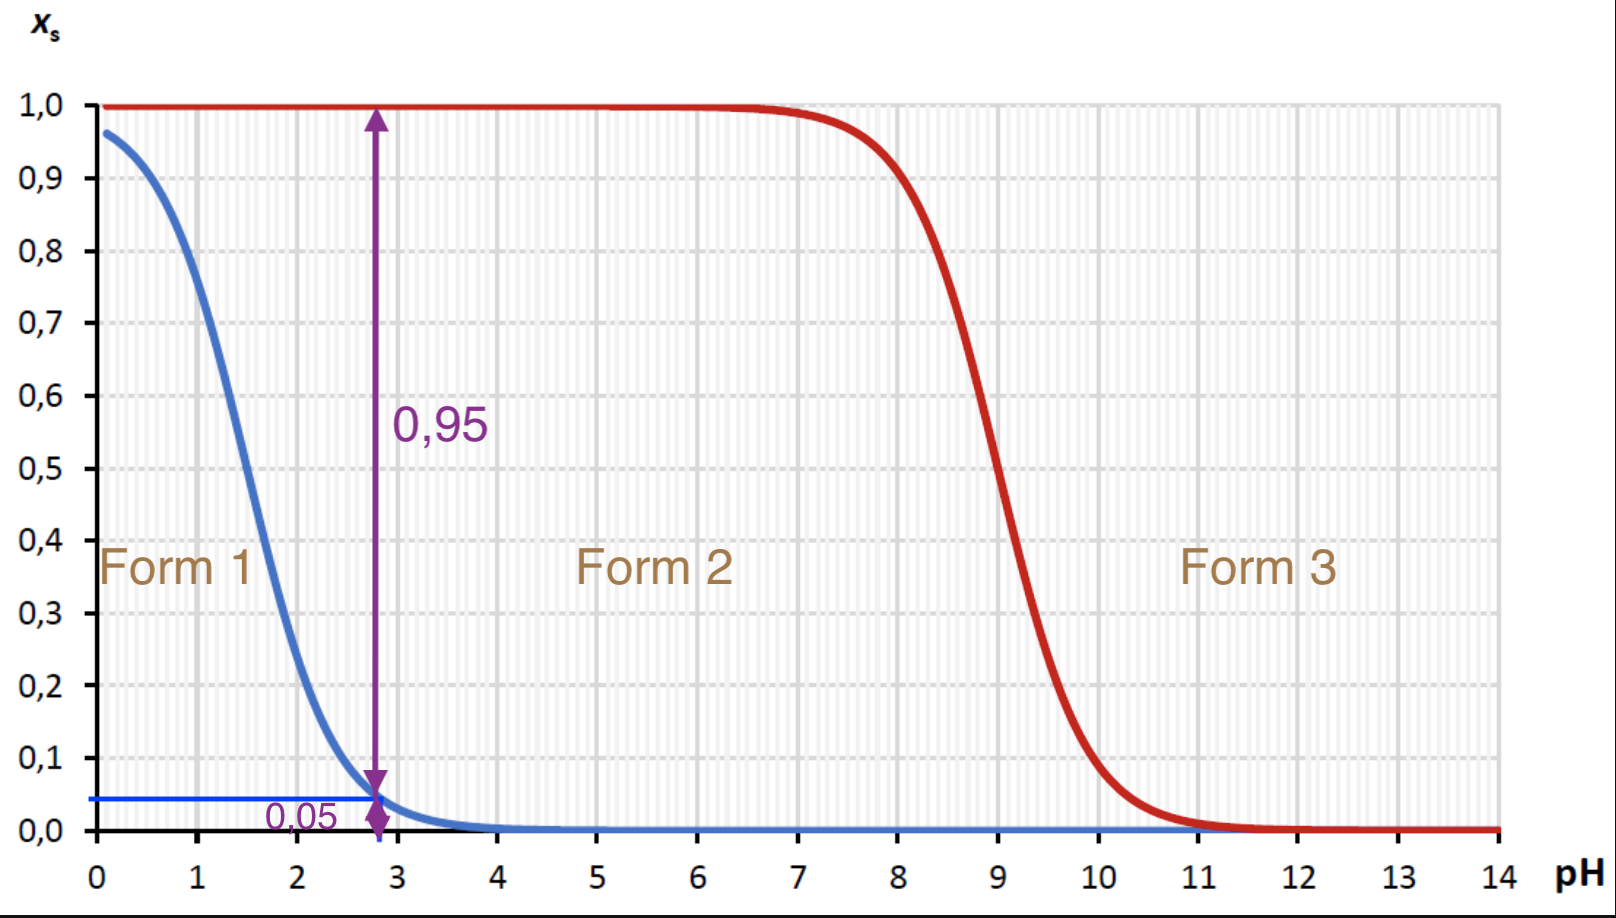
\includegraphics[width=\textwidth]{Bjerrum.png}
\end{center}
\caption{Aflæsning på bjerrumdiagrammet}
\label{fig:Bjerrum}
\end{figure}
\noindent \textbf{c.}
Hvis reaktionen er af første orden, så må der gælde, at
\begin{equation}
\begin{split}
v=k \cdot [\text{cystein} ]
\end{split}
  \label{eq:førsteorden}
\end{equation}
Det vil sige, at punkterne på $([\text{cystein} ], v)$-grafen skal ligge tilnærmelsesvist på en ret linje gennem (0,0).
Vi sætter da datapunkterne, hvor $[\text{cystein} ] < 10 \;\unit{\micro \textsc{m}} $ ind i Logger Pro og laver en ligefrem proportional regression, hvilket ses i \cref{fig:cystein}.
\begin{figure}[H]
\begin{center}
  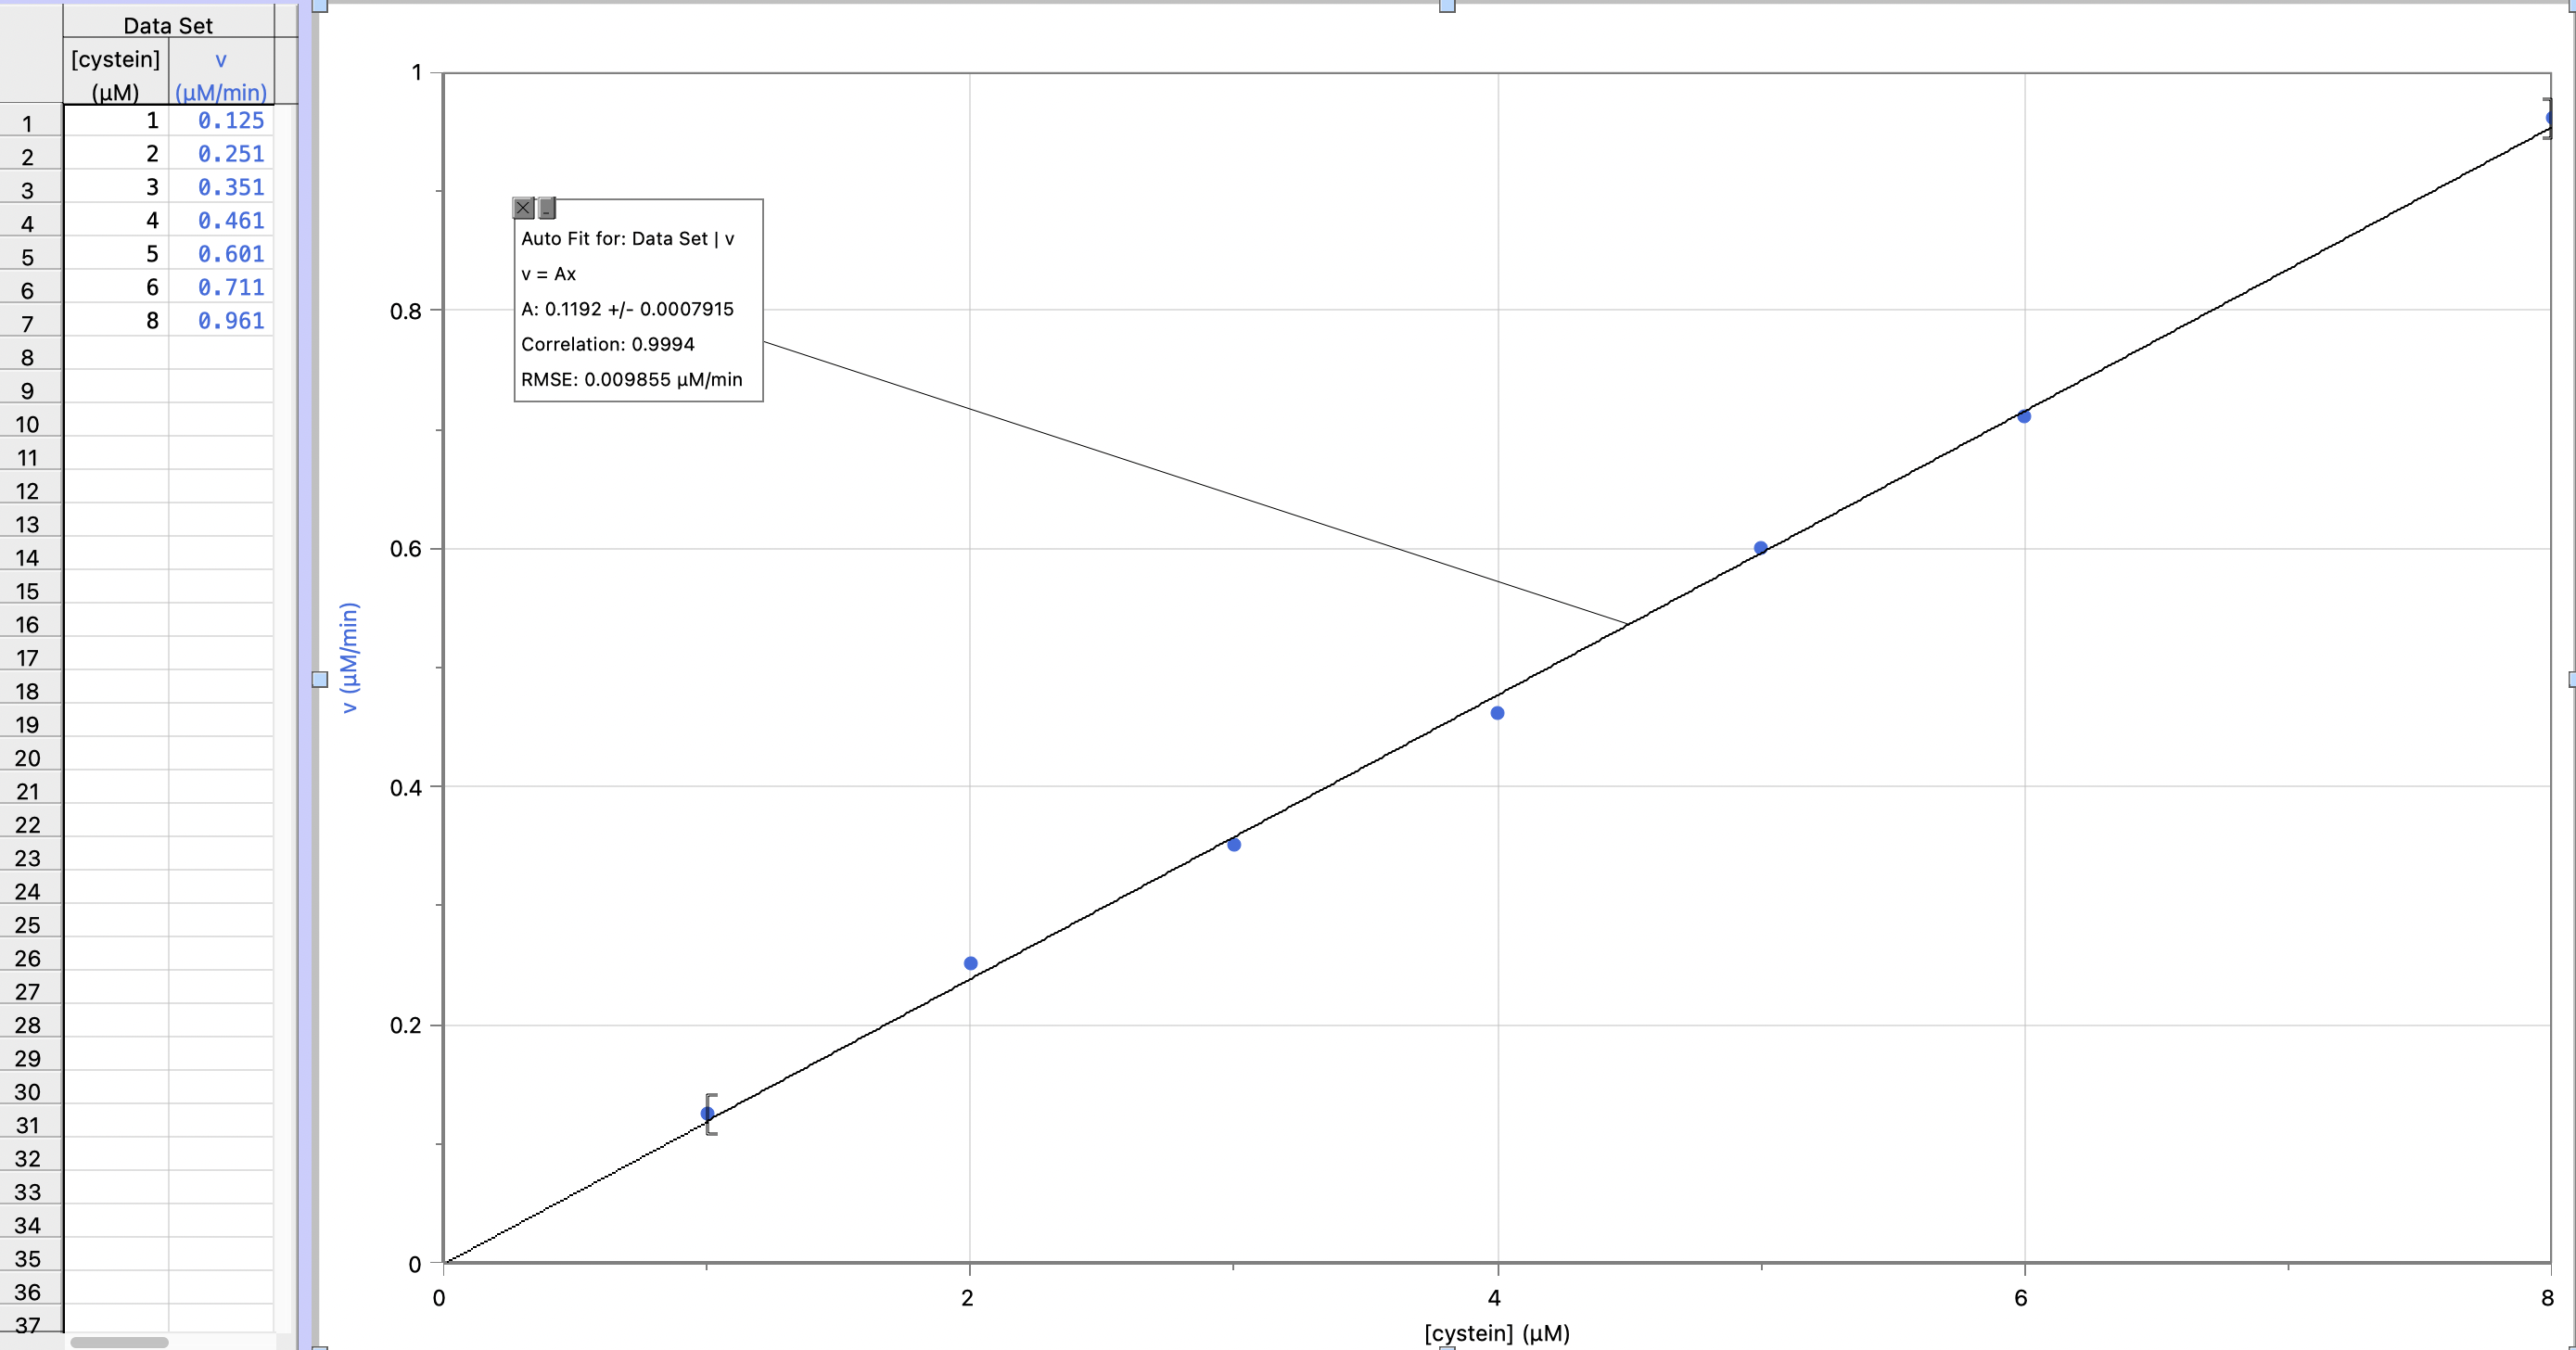
\includegraphics[width=\textwidth]{cystein.png}
\end{center}
  \caption{Ligefrem proportional regression på $([\text{cystein} ],v)$-grafen lavet i Logger Pro}
\label{fig:cystein}
\end{figure}
Det ses, at punkterne (hvor $[\text{cystein} ] < 10 \;\unit{\micro \textsc{m}} $) på $([\text{cystein} ], v)$-grafen ligger tilnærmelsesvist på en ret linje gennem (0,0), og reaktionen er altså af første orden.
Fra regressionen har vi, at 
\begin{equation*}
\begin{split}
  v=0,1192 \;\unit{min ^{-1}} \cdot [\text{cystein} ]
\end{split}
\end{equation*}
Sammenligner vi med ligning \ref{eq:førsteorden}, at hastighedskonstanten må være
\[
k=0,1192 \;\unit{min ^{-1}} \approx 0,119 \;\unit{min ^{-1}} 
\] 
Omdannelsen af cystein er altså af første orden for koncentrationer af cystein under $10 \;\unit{\micro \textsc{m}} $ med en hastighedskonstant på $k=0,119 \;\unit{min ^{-1}} $. 
\section*{Opgave 4 - Germanium}
\sol \\
\textbf{a.}
Fra de givne masseprocenter har vi, at der i $100 \;\unit{g} $ af argyrodit er
\begin{equation*}
\begin{split}
  n(\ce{Ag} )&=\frac{m(\ce{Ag} )}{M(\ce{Ag} )}=\frac{76,50 \;\unit{g} }{107,9 \;\unit{g/mol} }=0,70899 \;\unit{mol} \\
  n(\ce{Ge} )&=\frac{m(\ce{Ge} )}{M(\ce{Ge} )}=\frac{6,44 \;\unit{g} }{72,64 \;\unit{g/mol} }= 0,08866 \;\unit{mol} \\
  n(\ce{S} )&=\frac{m(\ce{S} )}{M(\ce{S} )}=\frac{17,06 \;\unit{g} }{32,07 \;\unit{g/mol} }= 0,53196 \;\unit{mol} 
\end{split}
\end{equation*}
Vi beregner nu stofmængdeforholdene.
\begin{equation*}
\begin{split}
  \frac{n(\ce{Ag} )}{n(\ce{Ge} )}&=\frac{0,70899 \;\unit{mol} }{0,08866 \;\unit{mol} } = 7,9970 \approx  8\\
  \frac{n(\ce{S} )}{n(\ce{Ge} )}&=\frac{0,53196 \;\unit{mol} }{0,08866 \;\unit{mol} } =  6,0002\approx 6
\end{split}
\end{equation*}
Det fremgår, at forholdet mellem stofmængderne af \ce{Ag}, Ge og \ce{S} med stor nøjagtihed er 8:1:6. 
Den empiriske formel for argyrodit må derfor være \ce{Ag8GeS6}. \\[1ex]
\textbf{b.}
Vi beregner tilvæksten i molar standard entropi for reaktionen.
\begin{equation*}
\begin{split}
  \Delta S \stst &= 2 \cdot S \stst(\ce{SO2(g)} ) + S \stst(\ce{GeO2(s)} ) - 3 \cdot S \stst (\ce{O2(g)} ) - S \stst (\ce{GeS2(s)} )\\
  &=2 \cdot 248,23 \;\unit{\frac{J}{mol \cdot K}} + 39,7 \;\unit{\frac{J}{mol \cdot K}} - 3 \cdot 205,15 \;\unit{\frac{J}{mol \cdot K}} - 87,9 \;\unit{\frac{J}{mol \cdot K}} \\
  &\approx -167 \;\unit{\frac{J}{mol \cdot K}} 
\end{split}
\end{equation*}
Vi bemærker, at $\Delta S \stst <0$, hvilket vil sige, at ordenen øges i retning fra venstre mod højre.
Dette er i overensstemmelse med reaktionsskemaet, hvor der er tre gasmolekyler på venstre side af reaktionspilen, hvor der kun er to på højre side, hvor antallet af faste stoffer forbliver konstant.
SKRIV SENERE

\textbf{c.}
Fra figuren har vi, at 
\begin{equation}
\begin{split}
\Delta G \stst =-0,1076 \;\unit{\frac{kJ}{mol \cdot K}} \cdot T +96,4 \;\unit{kJ/mol} 
\end{split}
\label{eq:DelG}
\end{equation}
Vi beregner nu den absolutte temperatur $T$.
\begin{equation*}
\begin{split}
  T&=\frac{t \cdot K}{\;\unit{\celsius} } + 273,15 \;\unit{K} \\
  &=\frac{500 \;\unit{\celsius} \cdot K}{\;\unit{\celsius} } + 273,15 \;\unit{K} \\
  &=773,15 \;\unit{K} 
\end{split}
\end{equation*}
Der gælder om tilvæksten i molar standard Gibbs-energi, at
\[
\Delta G \stst = -R \cdot T \cdot \ln\left(K\right) 
\] 
Kombinerer vi dette udtryk med ligning \ref{eq:DelG}, får vi 
\begin{equation}
\begin{split}
  -R \cdot T \cdot \ln\left(K\right) = -0,1076 \;\unit{\frac{kJ}{mol \cdot K}}  \cdot T + 96,4 \;\unit{kJ/mol} &\iff \ln\left(K\right) = \frac{0,1076 \;\unit{\frac{kJ}{mol \cdot K}} }{R} - \frac{96,4 \;\unit{kJ/mol} }{R \cdot T}\\
  &\iff K = e^{\frac{0,1076 \;\unit{\frac{kJ}{mol \cdot K}} }{R} - \frac{96,4 \;\unit{kJ/mol} }{R \cdot T}} 
\end{split}
\label{eq:K}
\end{equation}
For at bestemme enheden for ligevægtskonstanten $K$, opskriver vi ligevægtsloven for reaktionen.
\begin{equation*}
\begin{split}
  K=\frac{p(\ce{H2O})^2}{p(\ce{H2} )^2}
\end{split}
\end{equation*}
Det er da klart, at ligevægtskonstanten ikke har nogen enhed, og vi beregner den nu ved $T=773,15 \;\unit{K} $ med det fundne udtryk.
\begin{equation*}
\begin{split}
  K &= e^{\frac{0,1076 \;\unit{\frac{kJ}{mol \cdot K}} }{R} - \frac{96,4 \;\unit{kJ/mol} }{R \cdot T}}\\
  &=e^{\frac{0,1076 \cdot 10^3\;\unit{\frac{J}{mol \cdot K}} }{8,314 \;\unit{\frac{J}{mol \cdot K}} } - \frac{96,4 \cdot 10^3\;\unit{J/mol} }{8,314 \;\unit{\frac{J}{mol \cdot K}}  \cdot 773,15 \;\unit{K} }}\\
  &\approx 0,128
\end{split}
\end{equation*}
Ved $500 \;\unit{\celsius} $ er ligevægtskontanten altså $K=0,128$. 

Fra ligning \ref{eq:K} har vi, at når $T$ hæves, så bliver $\ln\left(K\right) $ større.
Når $\ln\left(K\right) $ bliver større, så bliver $K$ også større. 
Fra reaktionsskemaet ses det, at udbyttet af \ce{Ge(s)} øges, når $K$ bliver større (for så forskydes reaktionen mod højre).
Altså skal temperaturen hæves for at øge udbyttet af \ce{Ge(s)}.\\[1ex]
\textbf{d.}
Vi opstiller et SÆL-skema for ligevægten, hvilket ses i \cref{fig:SÆL}.
Vi betragter her kun gasserne, da det er dem, der indgår i ligevægtsloven.
\begin{table}[H]
  \centering
  \begin{tabular}{@{}llllll@{}}
  \toprule
    &\ce{GeO2(s) +} & \ce{2H2(g)} & \ce{->} & \ce{Ge(s) +} & \ce{2H2O(g)} \\
  \midrule
    Start & & $2,00 \;\unit{bar} $ & & & 0 \;\unit{bar} \\
    Ændring & & $-x$ & & & $x$ \\
    Ligevægt & & $2,00 \;\unit{bar} -x$ & & & $x$\\ 
  \bottomrule
  \end{tabular}
  \caption{SÆL-skema for reaktionen}
  \label{tab:SÆL}
\end{table}
Fra ligevægtsloven har vi så, at når ligevægtens har indstillet sig, så gælder
\begin{equation*}
\begin{split}
  K=\frac{p(\ce{H2O} )^2}{p(\ce{H2} )^2} &\implies 1,47 = \frac{x^2}{\left(2,00 \;\unit{bar} -x\right)^2}\\
  &\implies  x=1,09602 \;\unit{bar} 
\end{split}
\end{equation*}
Ligningen er løst for $x$ med CAS, hvilket ses i \cref{fig:CAS}.
Den anden løsning kan ikke bruges, da den giver et negativt partialtryk.
Fra idealgasloven har vi, at stofmængden af \ce{H2O}, når ligevægten har indstillet sig må være
\begin{equation*}
\begin{split}
  n(\ce{H2O} )&=\frac{p(\ce{H2O} ) \cdot V}{R \cdot T}
\end{split}
\end{equation*}
Da stofmængden af \ce{Ge} og \ce{H2O} er $0 \;\unit{mol} $ til start, og reaktionsforholdet mellem dem er 1:2, så må der gælde når ligevægten har indstillet sig, at
\begin{equation*}
\begin{split}
  n(\ce{Ge} )&=\frac{1}{2} \cdot n(\ce{H2O} )\\
  &=\frac{1}{2} \cdot \frac{p(\ce{H2O} ) \cdot V}{R \cdot T}\\
  &=\frac{1}{2} \cdot \frac{1,09602 \;\unit{bar} \cdot 1,00 \;\unit{L} }{0,0831 \;\unit{\frac{L \cdot bar}{mol \cdot K}} \cdot 923,15 \;\unit{K} }\\
  &=0,0071436 \;\unit{mol} 
\end{split}
\end{equation*}
For god ordens skyld udregner vi også stofmængden af \ce{GeO2} til start, for at se, at der virkeligt er et overskud af \ce{GeO2}.
\begin{equation*}
\begin{split}
  n(\ce{GeO2} )&=\frac{m(\ce{GeO2} )}{M(\ce{GeO2} )}\\
  &=\frac{2,10 \;\unit{g} }{104,59 \;\unit{g/mol} }\\
  &=0,020078 \;\unit{mol} 
\end{split}
\end{equation*}
Vi ser da, at siden $n(\ce{GeO2} )>n(\ce{Ge} )$, og reaktionsforholdet mellem dem er 1:1, så er der et overskud af \ce{GeO2}, og reaktionen kan forløbe.
Vi udregner nu massen af \ce{Ge}, når ligevægten har indstillet sig.
\begin{equation*}
\begin{split}
  m(\ce{Ge} )&=n(\ce{Ge} ) \cdot M(\ce{Ge} )\\
  &=0,0071436 \;\unit{mol} \cdot 72,64 \;\unit{g/mol} \\
  &\approx 0,519 \;\unit{g} 
\end{split}
\end{equation*}
Massen af germanium når ligevægten har indstillet sig er altså $m(\ce{Ge} )=0,519 \;\unit{g} $.
\begin{figure}[H]
\begin{center}
  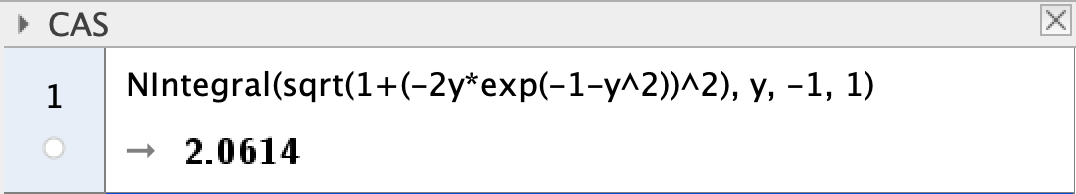
\includegraphics[width=0.6\textwidth]{CAS.png}
\end{center}
\caption{Ligningen løst med CAS}
\label{fig:CAS}
\end{figure}
\section*{Soltørring af vasketøj}
\sol \\
\textbf{b.}
Resultaterne fra test med 2,4-dinitrophenylhydrazin og Fehlings test ses i henholdsvis \cref{fig:dnph} og \cref{fig:Fehling}.
\begin{multicols}{2}
 \begin{figure}[H]
\begin{center}
  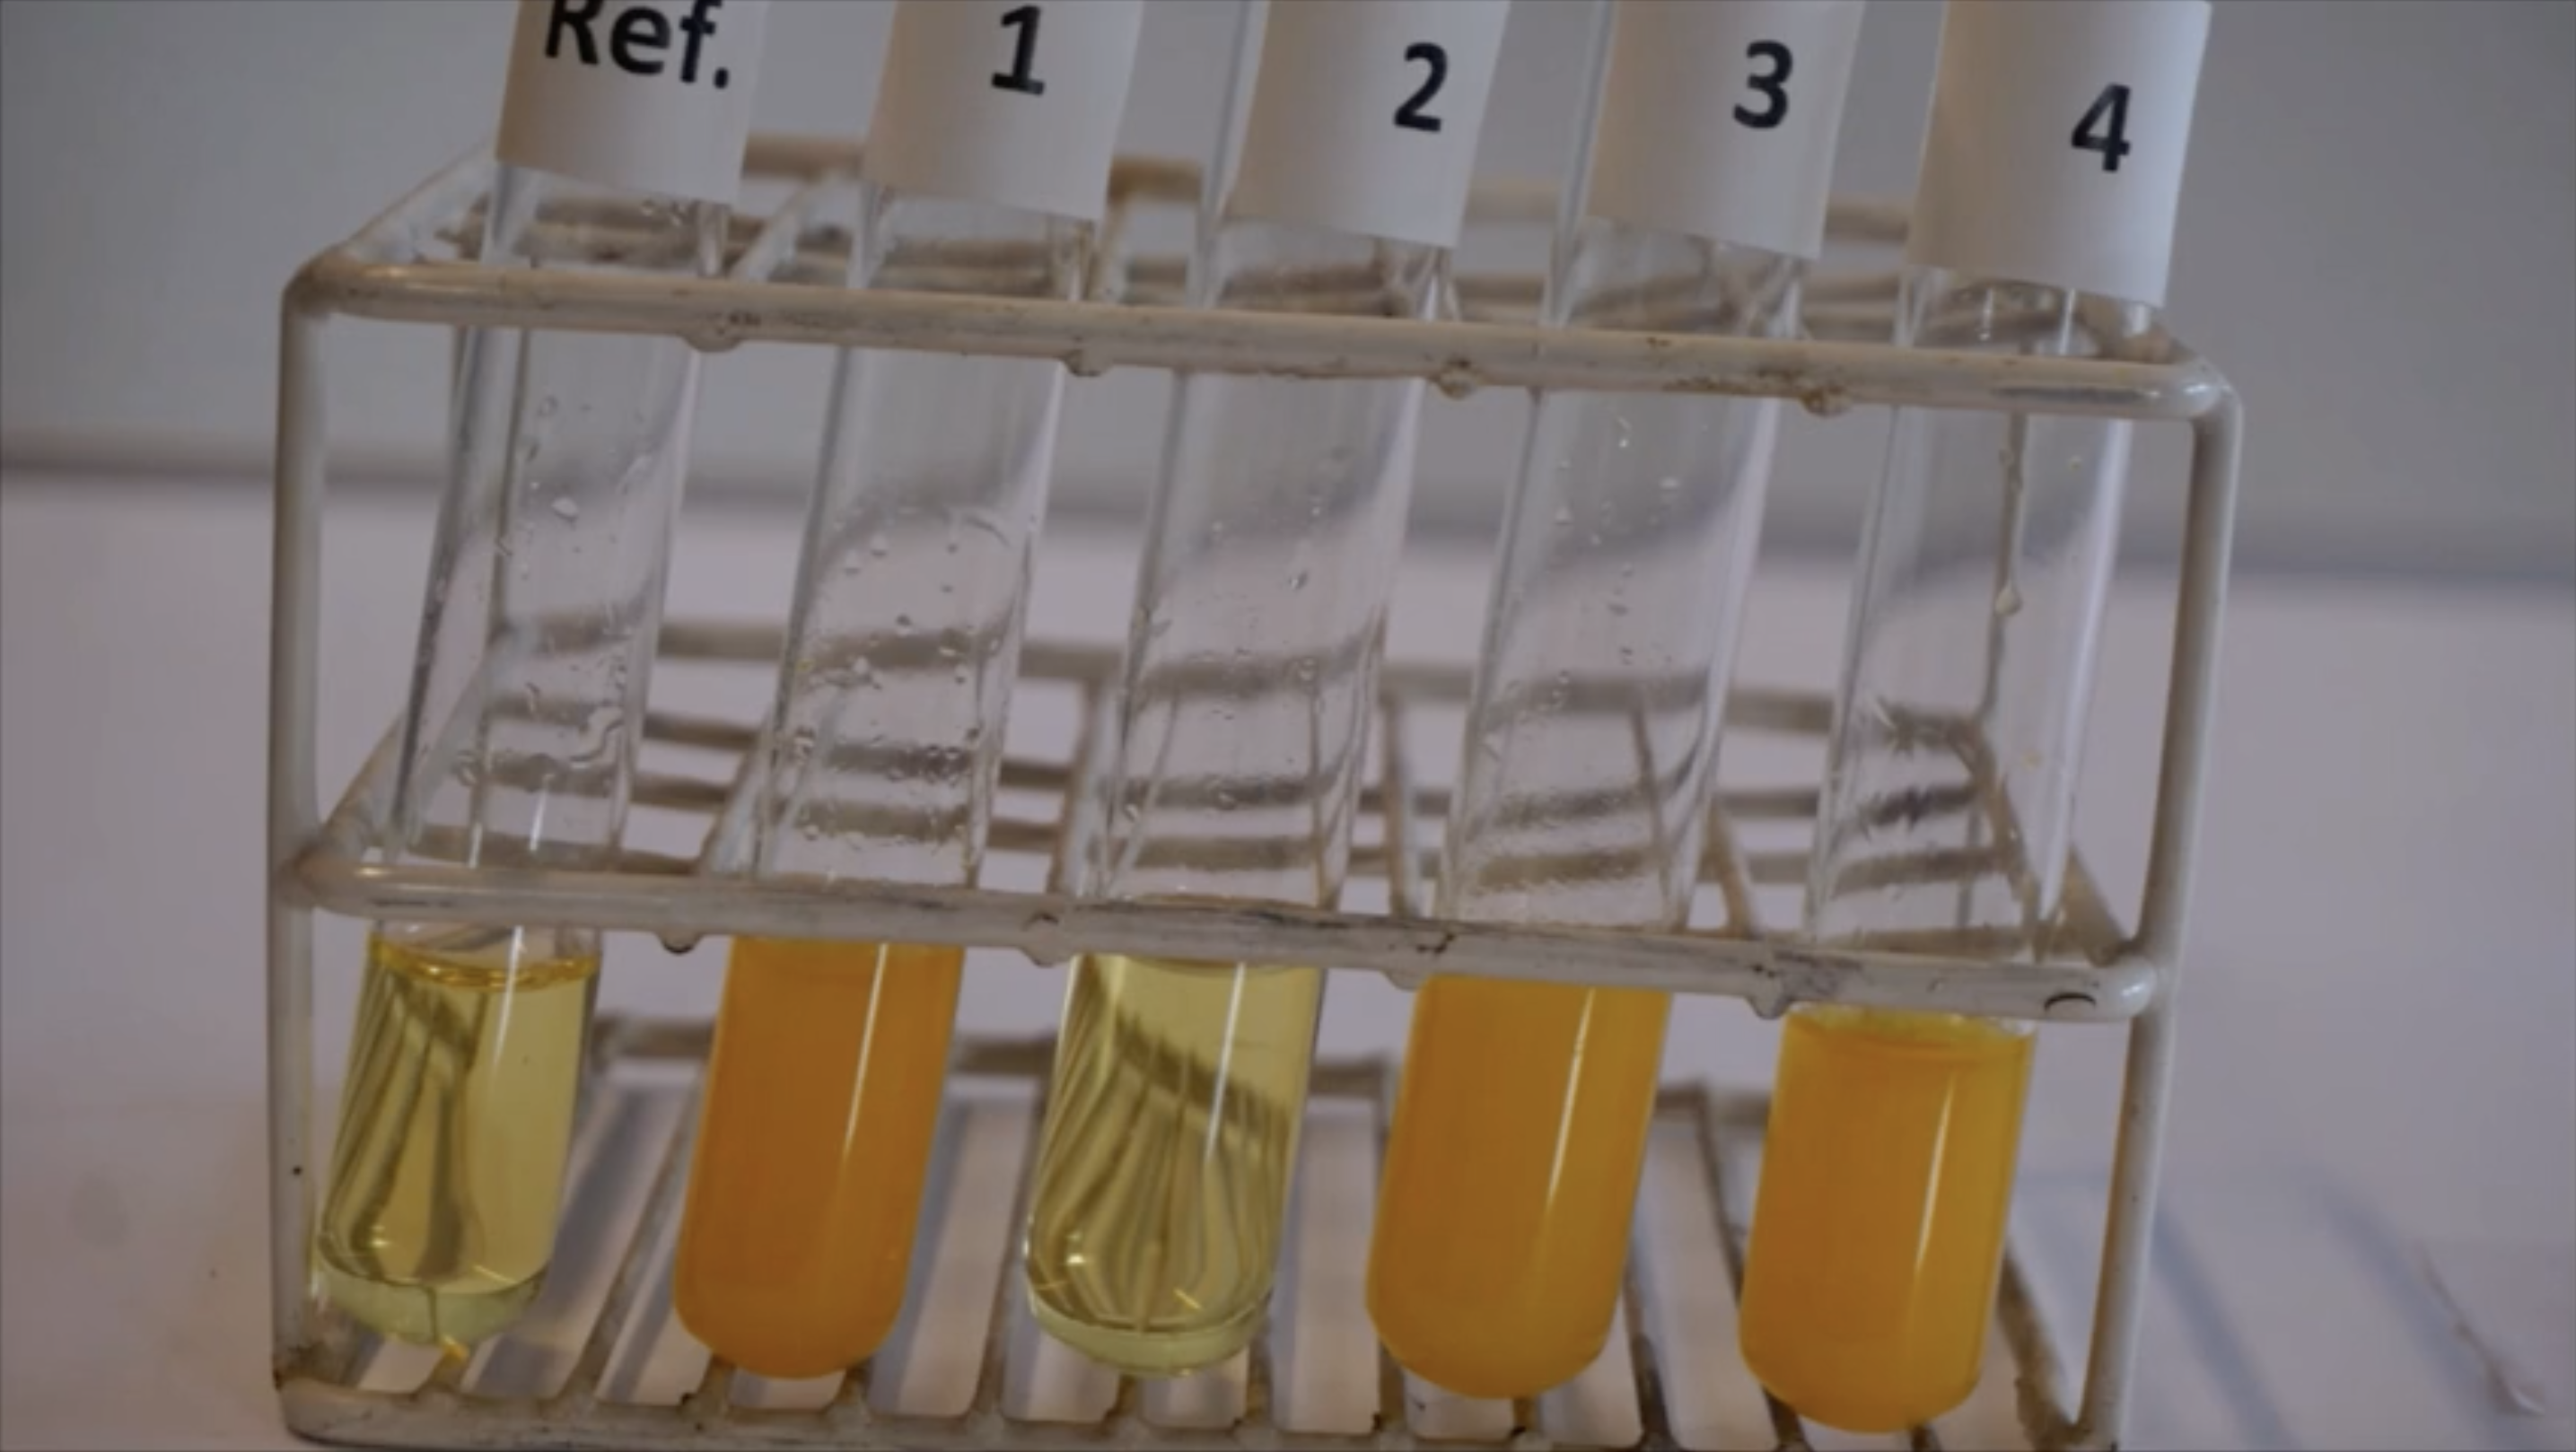
\includegraphics[width=0.5\textwidth]{dnph.png}
\end{center}
\caption{Resultater fra test med 2,4-dnph}
\label{fig:dnph}
\end{figure}
\begin{figure}[H]
\begin{center}
  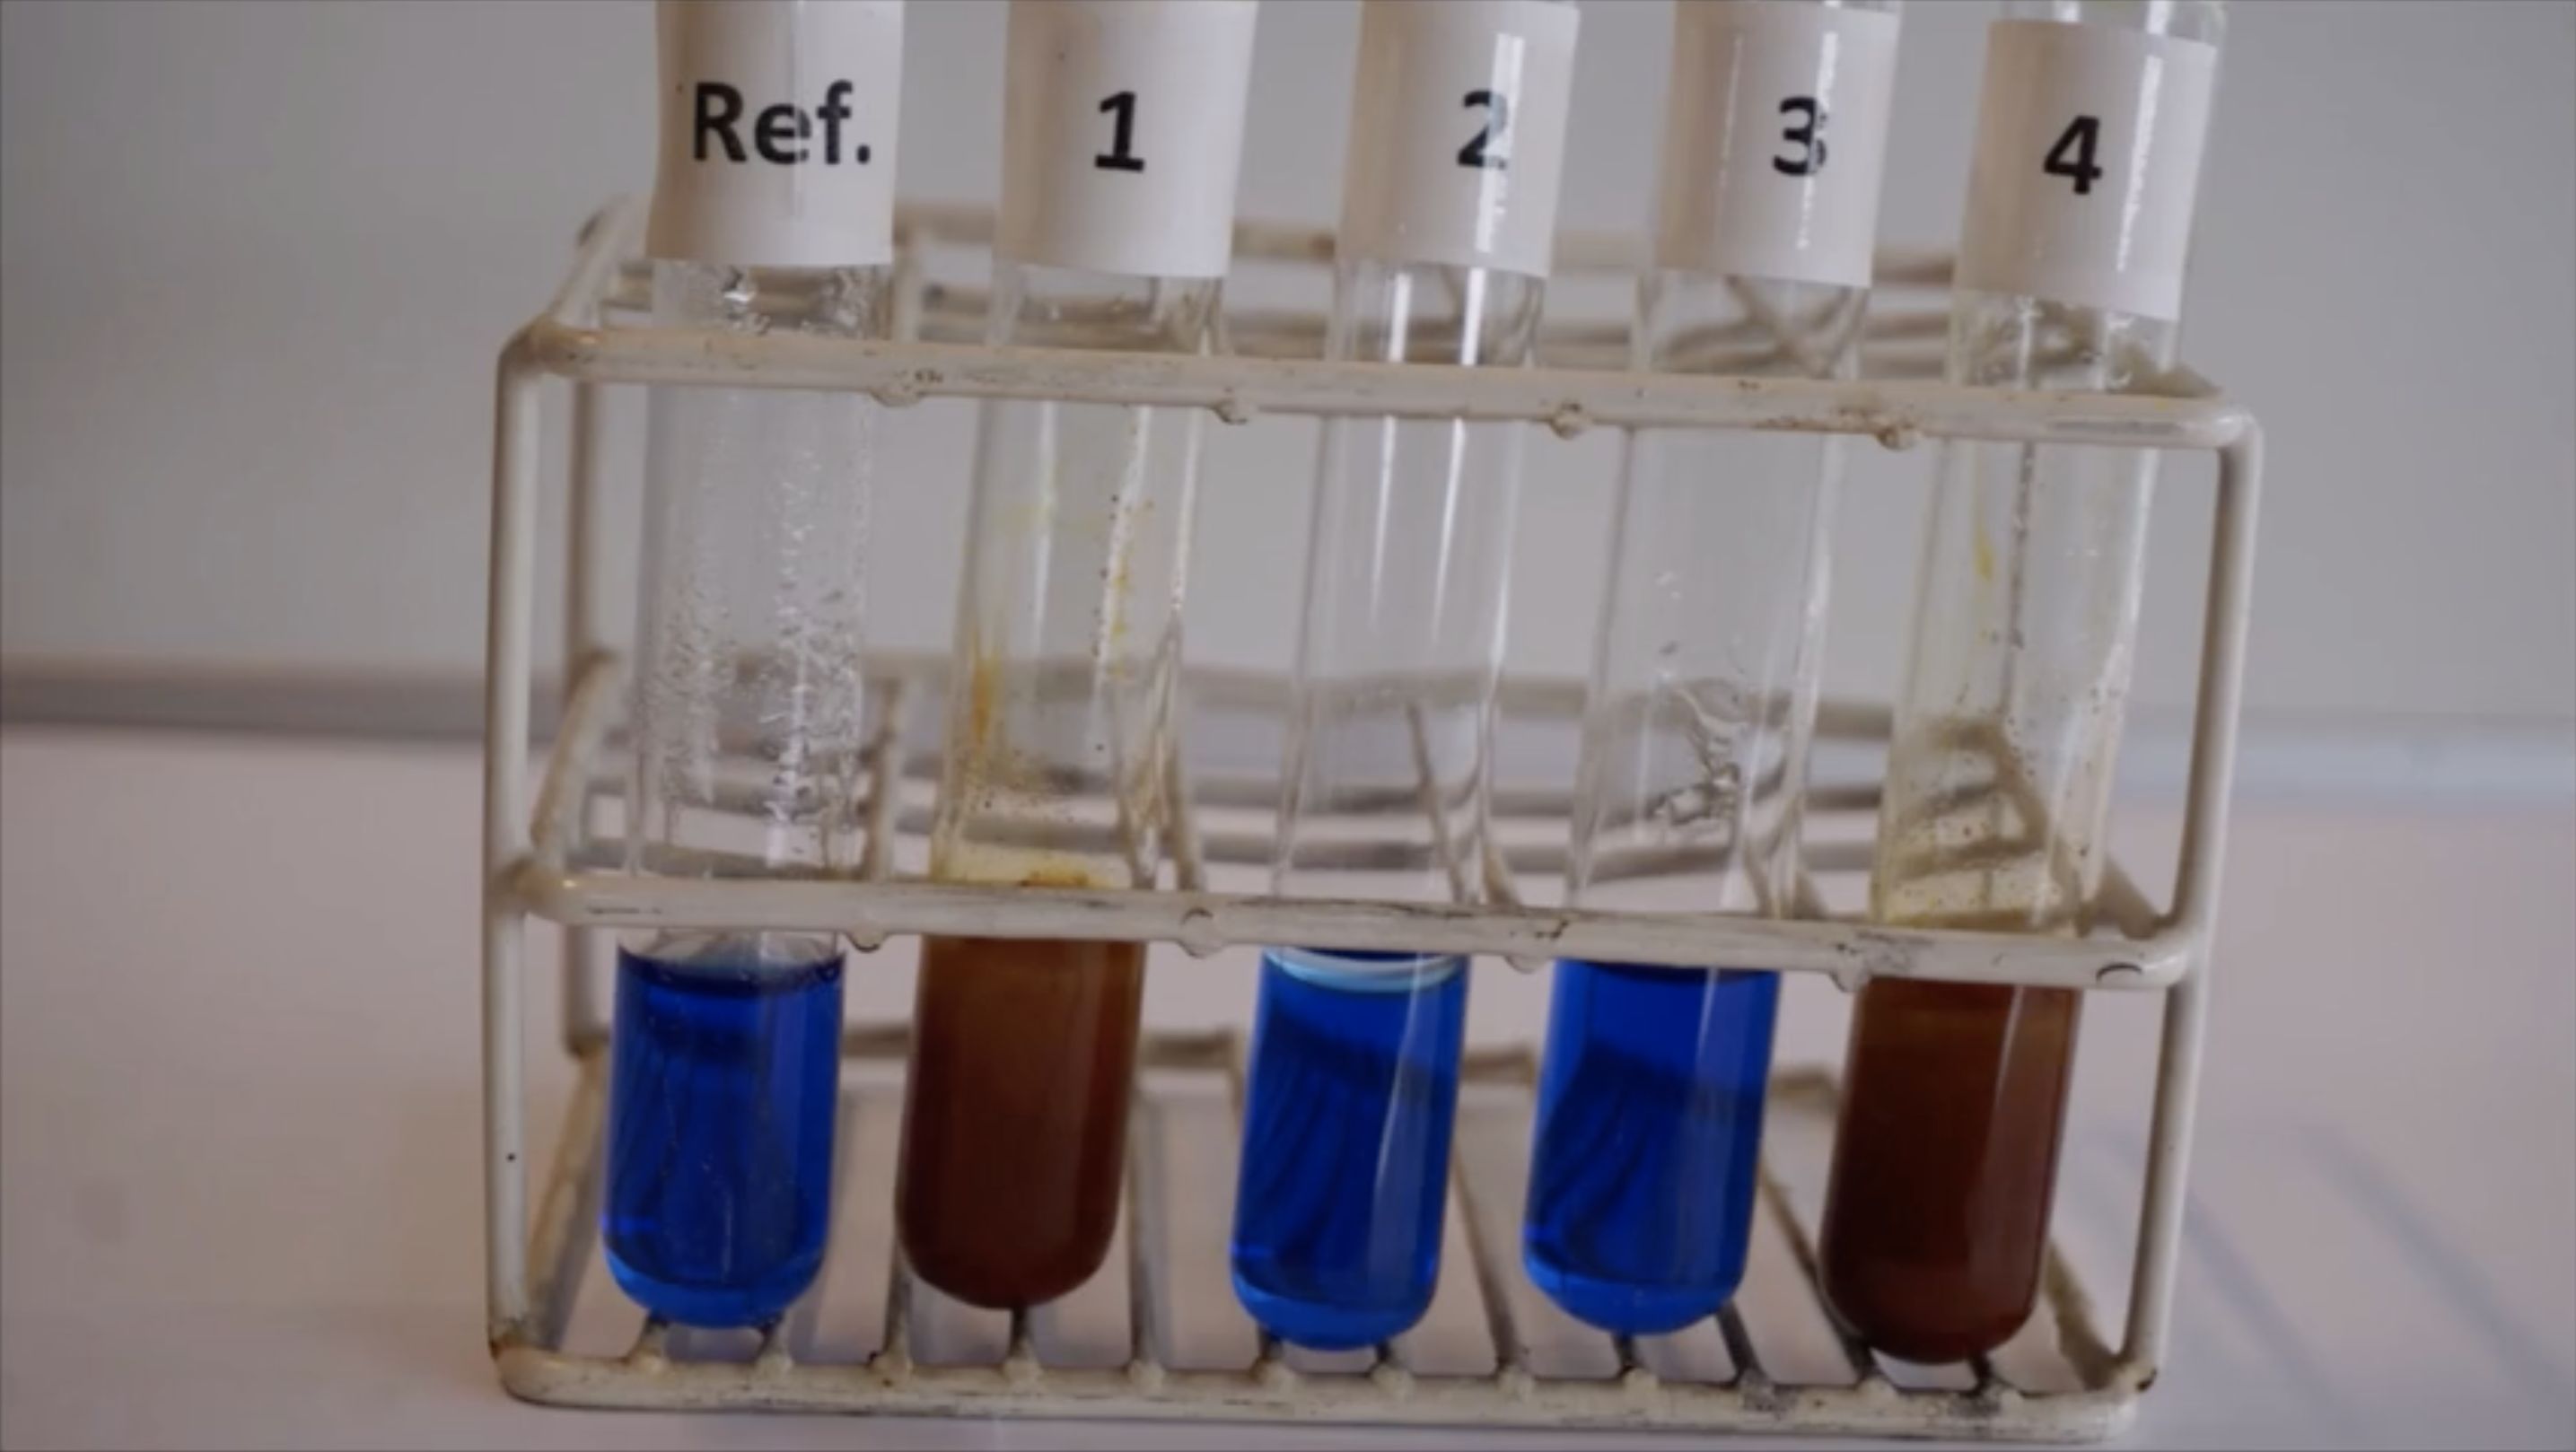
\includegraphics[width=0.5\textwidth]{Fehling.png}
\end{center}
\caption{Resultater fra Fehlings test}
\label{fig:Fehling}
\end{figure}
\end{multicols}
2,4-dinitrophenylhydrazin reagerer med både aldehyder og ketoner, hvor Fehlings test kun er positiv med aldehyder og som udgangspunkt ikke for ketoner.
Vi ser fra \cref{fig:dnph}, at stofferne i glas 1, 3 og 4 danner bundfald ved reaktion med 2,4-dinitrophenylhydrazin.
Altså må stofferne i disse være carbonylforbindelser.
Sammenligner vi med \cref{fig:BCDE}, ser vi, at det eneste stof, som ikke indeholder en carbonylgruppe er stof E, der er en alkohol (markeret med gul cirkel).
Stof E må altså være i glas 2.

I \cref{fig:Fehling} ser vi, at kun med stofferne i glas 1 og glas 4 dannes bundfald ved Fehlings test.
Siden stoffet i glas 3 danner bundfald ved reaktion med 2,4-dinitrophenylhydrazin men ikke ved Fehlings test, så må der være tale om en keton.
Fra \cref{fig:BCDE} ser vi, at stof C er den eneste keton blandt de fire stoffer (bemærk, at ketongruppen er markeret med blåt).
Altså må stof C være i glas 3.
Vi har nu tilordnet to af stofferne reagensglas alene på baggrund af de kemiske tests.
\begin{figure}[H]
\begin{center}
  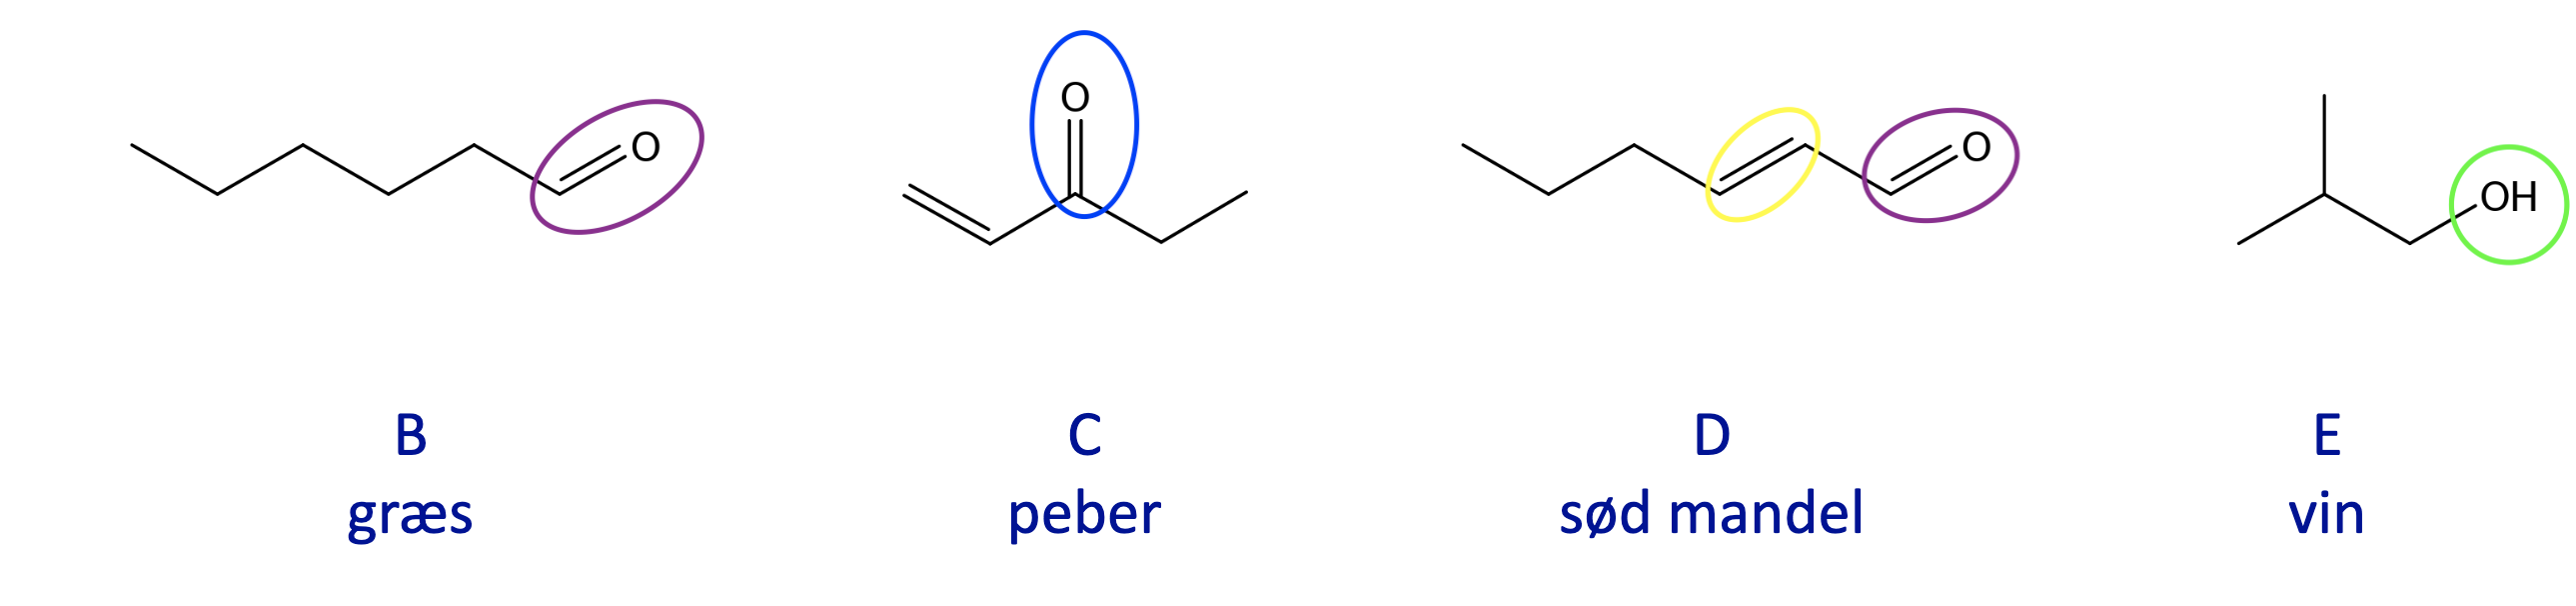
\includegraphics[width=\textwidth]{BCDE.png}
\end{center}
\caption{Strukturer for fire duftstoffer}
\label{fig:BCDE}
\end{figure}
Betragter vi de to resterende stoffer B og D ser vi, at stof D indholder en \ce{C=C}-binding, hvilket stof B ikke gør. 
I IR-spektret for stof D må der derfor være et absorptionsbånd for \ce{C=C} strækningsvibrationer, hvor \ce{C}-atomet er $sp^2$-hybridiseret. 
Dette bånd vil ligge ved bølgetallet $1600 \;\unit{cm ^{-1}}$ til $1700 \;\unit{cm ^{-1}}  $.

Betragter vi de to IR-spektre (\cref{fig:IR}), er det klart, at det første spektrum kan tilordnes stof D (se blå markering), og det andet spektrum kan tilordnes stof B.
\begin{figure}[H]
\begin{center}
  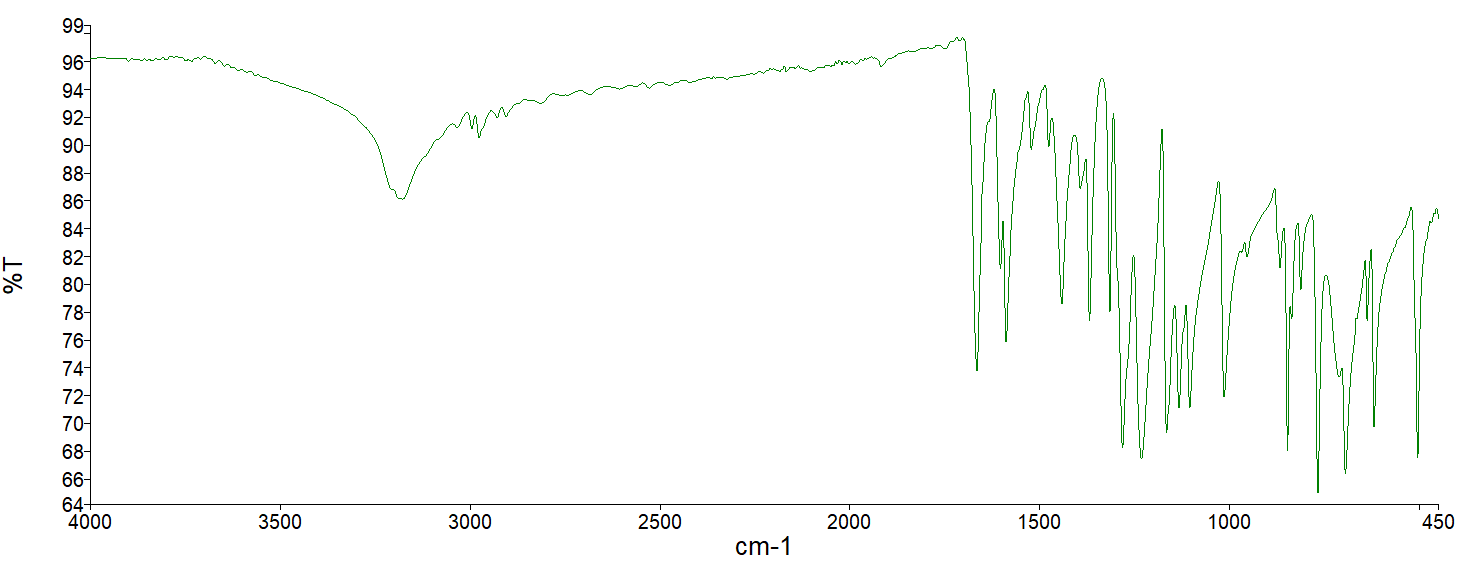
\includegraphics[width=0.6\textwidth]{IR.png}
\end{center}
\caption{IR-spektrene for henholdsvis stof D og stof B}
\label{fig:IR}
\end{figure}
\noindent \textbf{c.}
Vi vil starte med at bestemme den empiriske formel for F med udgangspunkt i elementaranalysen.
I $100 \;\unit{g} $ af stoffet F er der
\begin{equation*}
\begin{split}
  n(\ce{C} )&= \frac{69,72 \;\unit{g} }{12,01 \;\unit{g/mol} }=5,8052 \;\unit{mol} \\
  n(\ce{H} )&= \frac{11,70 \;\unit{g} }{1,008 \;\unit{g/mol} }=11,6071 \;\unit{mol} \\
  n(\ce{O} )&= \frac{18,57 \;\unit{g} }{16,00 \;\unit{g/mol} }=1,1606 \;\unit{mol} 
\end{split}
\end{equation*}
Vi beregner nu stofmængdeforholdene.
\begin{equation*}
\begin{split}
  \frac{n(\ce{C} )}{n(\ce{O} )}&=\frac{5,8052 \;\unit{mol} }{1,1606 \;\unit{mol} }=5,0018 \approx 5 \\
  \frac{n(\ce{H} )}{n(\ce{O} )}&=\frac{11,6071 \;\unit{mol} }{1,1606 \;\unit{mol} }= 10,0008 \approx 10
\end{split}
\end{equation*}
Forholdet mellem stofmængderne af \ce{C}, \ce{H} og \ce{O} er altså med stor nøjagtighed 5:10:1.
Den empiriske formel for \ce{F} er altså \ce{C5H10O}.
Vi kan nu udregne DBE for aldehydet (som er ens for alle molekyler med samme empiriske formel).
\begin{equation*}
\begin{split}
  DBE=\frac{(2 \cdot 5 + 2) - (10-0)}{2}=1 
\end{split}
\end{equation*}
Stof \ce{F} indeholder altså kun én dobbeltbindingsækvivalent, som må komme fra aldhyd-gruppen.

Vi betragter nu \ce{^1H}-NMR-spektret for \ce{F}.
En opsummerende tabel ses i \cref{tab:HNMR}.
\begin{table}[H]
\centering
\begin{tabular}{@{}lllllll@{}}
\toprule
  \makecell{Signal\\nr.} & \makecell{Kemisk skift\\(aflæst)\\$\delta$/ppm}& \makecell{Integral/areal\\(relativt antal ækvi-\\valente \ce{^1H}-atomer)}  & Opsplitning & \makecell{Antal nabo-\\\ce{^1H}'er}  & Tilordning & \makecell{Kemisk skift\\(tabel)\\$\delta$/ppm} \\
\midrule
  1 & 0,90 & 3 & Triplet & 2 & \ce{C\textbf{H}3-CH2 -}  & 0,9\\
  2 & 1,30 & 2 & Sekstet & 5 & \ce{-CH2-C\textbf{H}2-CH3} & 1,3 \\
  3 & 1,58 & 2 & Kvintet & 4 & \ce{-CH2-C\textbf{H}2-CH2-CHO} & 1,7\\
  4 & 2,41 & 2 & Kvartet & 3 & \ce{-CH2-C\textbf{H}2-CHO} & 2,5\\
  5 & 9,78 & 1 & Triplet & 2 & \ce{-CH2-C\textbf{H}O} & 9-10\\
\bottomrule
\end{tabular}
\caption{Tilordning af absorptionsbånd i \ce{^1H}-NMR-spektret for \ce{F} }
\label{tab:HNMR}
\end{table}
Der er fem signaler i spektret og dermed fem grupper af ækvivalente \ce{^1H}-kerner.
Det fremgår klart fra arealerne af signal nr. 1, 2, 3 og 4, at der må være én \ce{CH3}-gruppe og tre \ce{CH2}-grupper (pga. DBE).
Signal nr. 5 kan tilordnes \ce{CHO}-gruppen.

Fra opsplitningerne har vi så, at \ce{^1H}-kernerne hørende til signal nr. 2 må koble til \ce{^1H}-kernerne hørende til signal nr. 3. 
Derudover fremgår det også fra opsplitningerne, at \ce{^1H}-kernerne hørende til signal nr. 3 kobler til \ce{^1H}-kernerne hørende til signal nr. 2 og signal nr. 4, og at \ce{^1H}-kernerne hørende til signal nr. 4 også er koblet til \ce{^1H}-kernerne hørende til aldehydgruppen i signal nr. 5.

Altså vil det sige, at vi har \ce{CH3}-gruppen bundet til en \ce{CH2}-gruppe, der er bundet til en \ce{CH2}-gruppe, som er bundet til endnu en \ce{CH2}-gruppe, der er bundet til aldehydgruppen.
Strukturformlen for \ce{F} ses i \cref{fig:F}, hvor de \ce{^1H}-kerner, der svarer til hvert signal er numereret.
Vi ser, at dette er i overensstemmelse med den udregnede empiriske formel for \ce{F}.
\begin{figure}[H]
\begin{center}
  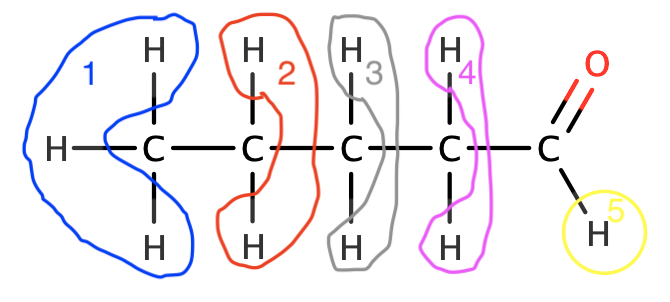
\includegraphics[width=\textwidth]{F.png}
\end{center}
\caption{Strukturformel for \ce{F} }
\label{fig:F}
\end{figure}

\end{document}
